\subsection{Estudio de mercado}


{\color{red}
\subsubsection*{Identificación del producto}

El producto es una innovadora plataforma de bienestar y entrenamiento personalizado, que proporciona a los nómadas digitales en Bogotá, y eventualmente en otras localidades, las herramientas y recursos para alcanzar y mantener un estilo de vida saludable. Este sistema interactivo se especializa en integrar el fitness personal con la vibrante vida cultural y las actividades físicas disponibles en la ciudad.

Las funcionalidades que ofrece la plataforma son las siguientes:

\begin{itemize}
    \item Cuenta personal registrada dentro del sistema: Los usuarios pueden registrarse y acceder con su usuario y contraseña para disfrutar de todas las funciones que el sistema brinda.
    
    \item Entrenamiento personalizado: Programas de ejercicio ajustados a los objetivos personales y preferencias de actividad, con la posibilidad de adaptarse a horarios y ubicaciones cambiantes.
    
    \item Seguimiento de progreso: Análisis detallado del rendimiento del usuario, con visualizaciones gráficas y seguimiento de indicadores de salud y fitness.
    
    \item Información de actividades locales: Un calendario interactivo y recomendaciones de eventos de fitness y bienestar que ocurren en Bogotá, permitiendo a los usuarios participar en la comunidad local.
    
    \item Integración comunitaria: Oportunidades para la interacción social y la construcción de redes a través de eventos grupales y actividades al aire libre.
    
\end{itemize}

\subsubsection*{Demanda}

El proyecto se dirige a atender la demanda creciente de nómadas digitales y profesionales remotos en Bogotá que buscan integrar el bienestar y la actividad física en sus vidas dinámicas y móviles. Esta población objetivo valora la flexibilidad y personalización en sus opciones de fitness, y busca soluciones que se ajusten a su estilo de vida nómada, sin estar ligados a una ubicación fija. 

Además, el proyecto busca satisfacer la necesidad de conexión social y cultural mediante la inclusión de actividades físicas locales, atendiendo así a la demanda de experiencias enriquecedoras y auténticas que complementen la vida profesional activa. 

\subsubsection*{Oferta}

Considerando la demanda identificada y el análisis de precio que se desarrollará posteriormente, se compara la oferta con la de los competidores para resaltar las ventajas únicas de la plataforma. Estas ventajas se traducen en un valor agregado significativo para los usuarios, como:

\begin{itemize}
    \item Una experiencia de usuario personalizada que integra programas de entrenamiento adaptativos con eventos de bienestar y actividades culturales en Bogotá, facilitando un estilo de vida saludable y socialmente activo.
    
    \item Una interfaz que no solo permite a los usuarios gestionar sus rutinas de ejercicio, sino también descubrir y conectarse con eventos locales de fitness, proporcionando una solución integral para la vida nómada.
    
    \item La función de calendario comunitario que ofrece recomendaciones basadas en las preferencias y el historial de actividad de los usuarios, incentivando la participación en la comunidad local de fitness y bienestar.
\end{itemize}

\subsubsection*{Plan de marketing}

La implementación de estrategias de marketing es crucial para el éxito del proyecto, especialmente en las etapas iniciales, donde el objetivo principal es alcanzar a la audiencia objetivo y construir una imagen de marca sólida. A través del marketing, el proyecto busca no solo ganar reconocimiento en el mercado de Bogotá y posteriormente a nivel global, sino también consolidar una base de clientes leales.

\textbf{Objetivos}
\begin{itemize}
    \item Lanzar la plataforma al mercado, destacando su propuesta única de valor que integra entrenamiento personalizado y actividades físicas en Bogotá adaptadas a los nómadas digitales.
    \item Alcanzar una acogida positiva entre el público objetivo a través de campañas de marketing enfocadas y personalizadas.
    \item Fidelizar a los usuarios mediante una experiencia de usuario excepcional, contenido de valor y una comunidad activa y de apoyo.
    \item Posicionarse como líder en el mercado de bienestar digital para nómadas digitales en Bogotá, con planes de expansión nacional e internacional.
    \item Maximizar los ingresos a través de la retención de clientes y la adquisición de nuevos usuarios, empleando estrategias de marketing digital y colaboraciones estratégicas.
\end{itemize}

\textbf{Táctica}

El presente proyecto adoptará estrategias de marketing digital innovadoras, aplicando un enfoque de inbound marketing para atraer y retener a nómadas digitales interesados en mejorar su bienestar y estilo de vida activo. A diferencia del marketing tradicional, que interrumpe al consumidor, el marketing digital entrante se centra en ser descubierto orgánicamente por aquellos que buscan soluciones activamente, ofreciendo contenido útil y relevante en cada etapa del viaje del consumidor. \cite{Opreana2015}

El inbound marketing se caracteriza por:

\begin{itemize}
    \item \textbf{Transformación del Marketing:} Reconociendo que el marketing tradicional ha perdido efectividad, este proyecto se enfoca en atraer consumidores mediante el uso estratégico de contenido valioso, posicionándose donde los consumidores ya están buscando soluciones.
    
    \item \textbf{Estrategias Online:} Se implementarán comunicaciones de marketing centradas en la marca, aprovechando el marketing de contenidos, las redes sociales y la optimización de motores de búsqueda (SEO) para mejorar la visibilidad y el alcance.
    
    \item \textbf{Marketing vs. Marketing Digital Entrante:} Mientras el marketing tradicional busca captar la atención por interrupción, nuestro enfoque estará en atraer a los consumidores de manera natural, ofreciéndoles soluciones y contenido de valor justo cuando lo necesitan.
    
    \item \textbf{Medición del Marketing Digital Entrante:} La efectividad de nuestras estrategias digitales se medirá analizando la actividad del sitio web, las fuentes de tráfico, el comportamiento de los visitantes y los resultados obtenidos, permitiéndonos ajustar nuestras tácticas para maximizar el impacto.
\end{itemize}

El objetivo es crear un ciclo virtuoso donde los nómadas digitales no solo encuentren en nuestra plataforma un recurso valioso para su salud y bienestar, sino que también se conviertan en promotores activos de nuestra marca, gracias a la calidad y relevancia del contenido y las experiencias que ofrecemos.

Como se aprecia en la Figura \ref{inboundMarketing} sobre inbound marketing, se detallan las etapas claves que se seguirán para garantizar el éxito del proyecto y la satisfacción de nuestros usuarios:

\vspace{2mm}
        \begin{minipage}{0.9\textwidth}
        \centering
        \captionof{figure}[{Fases Inbound Marketing}]{ Fases Inbound Marketing  }
        \label{inboundMarketing}
         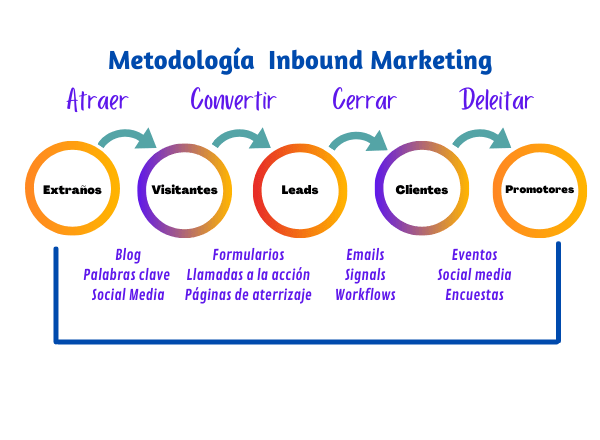
\includegraphics[width=0.8\textwidth]{Content/Images/Metodologia-Inbound-Marketing.png}
        \footnote{Nota. \textup{Fuente: Inbound Marketing, la guía completa \cite{EstudioTurismoenterritoriosruralesdeBogotá}}}  
\end{minipage}


\begin{itemize}
    \item \textbf{Atraer:} La primera etapa se enfoca en atraer a los nómadas digitales interesados en un estilo de vida saludable mediante contenido relevante y de alta calidad. Utilizaremos blog posts, guías, infografías y videos que respondan a sus preguntas y necesidades, promovidos a través de SEO y redes sociales para aumentar nuestra visibilidad.
    
    \item \textbf{Convertir:} Una vez atraídos a nuestro sitio, el objetivo es convertir a esos visitantes en leads. Esto se logrará ofreciendo recursos valiosos como ebooks, webinars y newsletters a cambio de su información de contacto, utilizando formularios optimizados y llamadas a la acción (CTAs) claras y atractivas.
    
    \item \textbf{Cerrar:} En esta etapa, trabajaremos para convertir a los leads en usuarios de nuestra plataforma. Utilizaremos email marketing personalizado y automatización de marketing para nutrir a estos leads con contenido específico basado en sus intereses y comportamientos, guiándolos suavemente hacia la decisión de compra.
    
    \item \textbf{Deleitar:} El trabajo no termina con la conversión. La última etapa se centra en fidelizar a estos usuarios, convirtiéndolos en promotores de nuestro proyecto. Esto incluye ofrecerles contenido continuo, soporte excepcional y oportunidades de participación, como foros y comunidades, para mantenerlos comprometidos y satisfechos.
\end{itemize}

Este enfoque no solo nos permite conectar de manera más efectiva con nuestros usuarios sino también crear una base sólida de clientes leales que ayudarán a promover nuestro proyecto a través de sus redes, amplificando nuestro alcance de manera orgánica y sostenible.



\subsubsection*{Precio}

Teniendo en cuenta la variedad de servicios de bienestar y entrenamiento personalizado, así como las características únicas de la solución ofrecida comparada con las alternativas disponibles en el mercado, el precio de la plataforma de bienestar y fitness para nómadas digitales ha sido calculado teniendo en cuenta los siguientes factores:

\begin{itemize}
    \item Fidelización de clientes: Creando un valor agregado que justifique la retención y satisfacción a largo plazo.
    \item Optimización de los beneficios a corto y largo plazo: Asegurando la sostenibilidad financiera del proyecto.
    \item Incursión eficaz y eficiente en el mercado: Posicionando competitivamente el servicio en el ecosistema digital.
    \item Costos de mantenimiento: Cubriendo los gastos operativos de la plataforma sin comprometer la calidad.
    \item Producto similar en la competencia: Analizando y comparando para establecer un precio competitivo.
    \item Demanda del servicio: Evaluando la disposición a pagar de los nómadas digitales por soluciones de bienestar personalizadas.
    \item Soporte técnico: Incluyendo el costo de ofrecer un soporte al cliente excepcional y personalizado.
\end{itemize}

\begin{adjustbox}{
            center,
            caption=[{Precio en el mercado actual}]{\centering Precio en el mercado actual (Valores en pesos colombianos COP). },
            label={Precio},
            nofloat=table, vspace={20px}}
            {
            \begin{threeparttable}
           \begin{tabular}{|p{11cm}|p{10cm}p{2cm}|}
                \hline
                \rowcolor[HTML]{D9EAD3} 
                \cellcolor[HTML]{D9EAD3}                              & \multicolumn{2}{c|}{\cellcolor[HTML]{D9EAD3}Precio}            \\ \cline{2-3} 
                \rowcolor[HTML]{D9EAD3} 
                \multirow{-2}{*}{\cellcolor[HTML]{D9EAD3}Suscripción} & \multicolumn{1}{l|}{\cellcolor[HTML]{D9EAD3}Mínimo} & Máximo   \\ \hline
                \multicolumn{1}{|l|}{Mensualidad}                     & \multicolumn{1}{l|}{\$70000}                       & \$270000 \\ \hline
            \end{tabular}
            \begin{tablenotes}[para,flushleft]
                \vspace{2mm}
               \textit Nota. Fuente: Autores.
            \end{tablenotes}
            
        \end{threeparttable} 
    }        
            
\end{adjustbox}

Si bien los precios que existen actualmente en el mercado son bastante competitivos y sus modelos de negocio muy similares, el factor diferencial de nuestro proyecto radica en su asequible precio de suscripción mensual y el cobro por comisión por participantes en actividades y eventos exitosos, lo cual se espera proporcione la mayor cantidad de ingresos. Nuestro modelo de negocio contará tanto con un servicio de suscripción por periodos como se muestra a continuación:

\begin{adjustbox}{
            center,
            caption=[{Precios de suscripción.}]{Precios de suscripción mensual y publicidad. },
            label={PrecioPeriodos},
            nofloat=table, vspace={20px}}
            {
            \begin{threeparttable}
           \begin{tabular}{|p{7.8cm}|p{7.8cm}|}
            \hline
            \rowcolor[HTML]{D9EAD3} 
            Suscripción & Precio       \\ \hline
            Mensualidad & \$ 50.000    \\ \hline
            Publicidad   & \$ 100.000   \\ \hline
            %Anualidad   & \$ 800.000 \\ \hline
            \end{tabular}%
            
            \begin{tablenotes}[para,flushleft]
                \vspace{2mm}
                \textit Nota. Fuente: Autores.
            \end{tablenotes}
            
        \end{threeparttable} 
    }        
            
\end{adjustbox}
}